\documentclass[12pt]{article}
\usepackage[pdftex]{graphicx}

\usepackage[english]{babel}
\usepackage[utf8x]{inputenc}
\usepackage{amsmath}
\usepackage{graphicx}
\usepackage[colorinlistoftodos]{todonotes}
\usepackage{fancyhdr}

\lhead{Sharing Framework}
\rhead{Intermediate Report}
\setlength{\headheight}{15.0pt}
\pagestyle{fancy}

\title{Sharing Framework: Intermediate Report}
\author{Chris Spalding\\Ian Saad\\Greg Finch\\Wesley Stedman\\Bobby Kearns}

\begin{document}
\begin{titlepage}
\maketitle
\end{titlepage}

\section{Design Specification}

\subsection{Walkthrough of our code}

We will likely use a Singleton design pattern for our database. This is mainly because we only need a single database class to keep track of all of the users' information.

The code for the database will be pretty basic. The script will access the server by logging in and from there the code will instantiate a database that will hold the files. The code will then create tables that will contain different files. There will be a table that holds user account information, a table that holds saved projects created by the user, and images that are used in the project. For the project table there will be unique keys that link that specific project to the user that created so that when the user loads that file the server will know where that file is because the key is associated with the user calling it. This will work the same way when the user is trying to share the project as well.

\subsection{Design Rationale}

We chose to use the singleton pattern because we will have only one instance of the database operating.  No other design pattern would apply because our part of the system can only operate as a single entity and will only be represented by one class.

\subsection{Interfaces}

Our system provides other teams with the ability to load and save to a database. Teams will have to use a loadFile command to load a file from the database. Also provided are saveFile, shareFile, and Login commands. Login is required before loading or saving can occur. This allows us to distinguish between users when saving files. This also allows us to prevent users from accessing other files.

The user will not be directly interacting with us. They will being using elements in the gui that will call our provided methods to accomplish tasks with the server. 

\subsection{Design Details and Restrictions}

We are partially restricted by other groups and their styles/implementation; need to know exactly what we will be called for. Overall our module has fairly specific operations that have rather straightforward designs. We have a database that will “guide” us on how we implement storing and retrieving information from it.


\section{Project Status}

We currently have the skeleton for a database. We need to implement load, save, and share methods. In order to do that we need to talk to a few groups to make sure we know what type of file to save/share. After implementing these three methods, the last step for our group will be to effectively put the other groups’ code ‘on top’ of ours. We’ll have to allow the other groups to access our database so that user’s will be able to save, share, and load their projects without seeing the inner workings of the server.

\subsection{Member Duties}
Ian is working on saving files. This means that he will be working on making a save method within our database. Greg's main duty is making a method to facilitate file sharing between users. Chris' main duty has been to write Latex code, but moving forward he will help to facilitate group communication as well as debugging and helping everyone with miscellaneous coding needs. Wesley will work on creating a file loading method that is easy to use, and Bobby's task will be to work on user authentication.

\subsection{Timeline for Implementation}
While every member of our team will be involved in each part of the module, we have divided the work into the methods involved with the database. Greg will be focused primarily on file sharing, Wesley on file loading, Bobby on user authentication, Ian on file saving, and Chris being the floating member and \LaTeX expert. 

After the server is set up, all the functions can be worked on simultaneously to some extent, so we have layed them out as such. For the first Integration Day we will have save and load completed as they are fairly similar and are the core functionality of our module. These two functions also allow the other modules to do most of what they need from us. When those are completed, the working members will move to assist on log on and share. For the second Integration Day we will have log on completed and before the final day, share will be complete.
\newpage

\begin{figure}
 \centerline{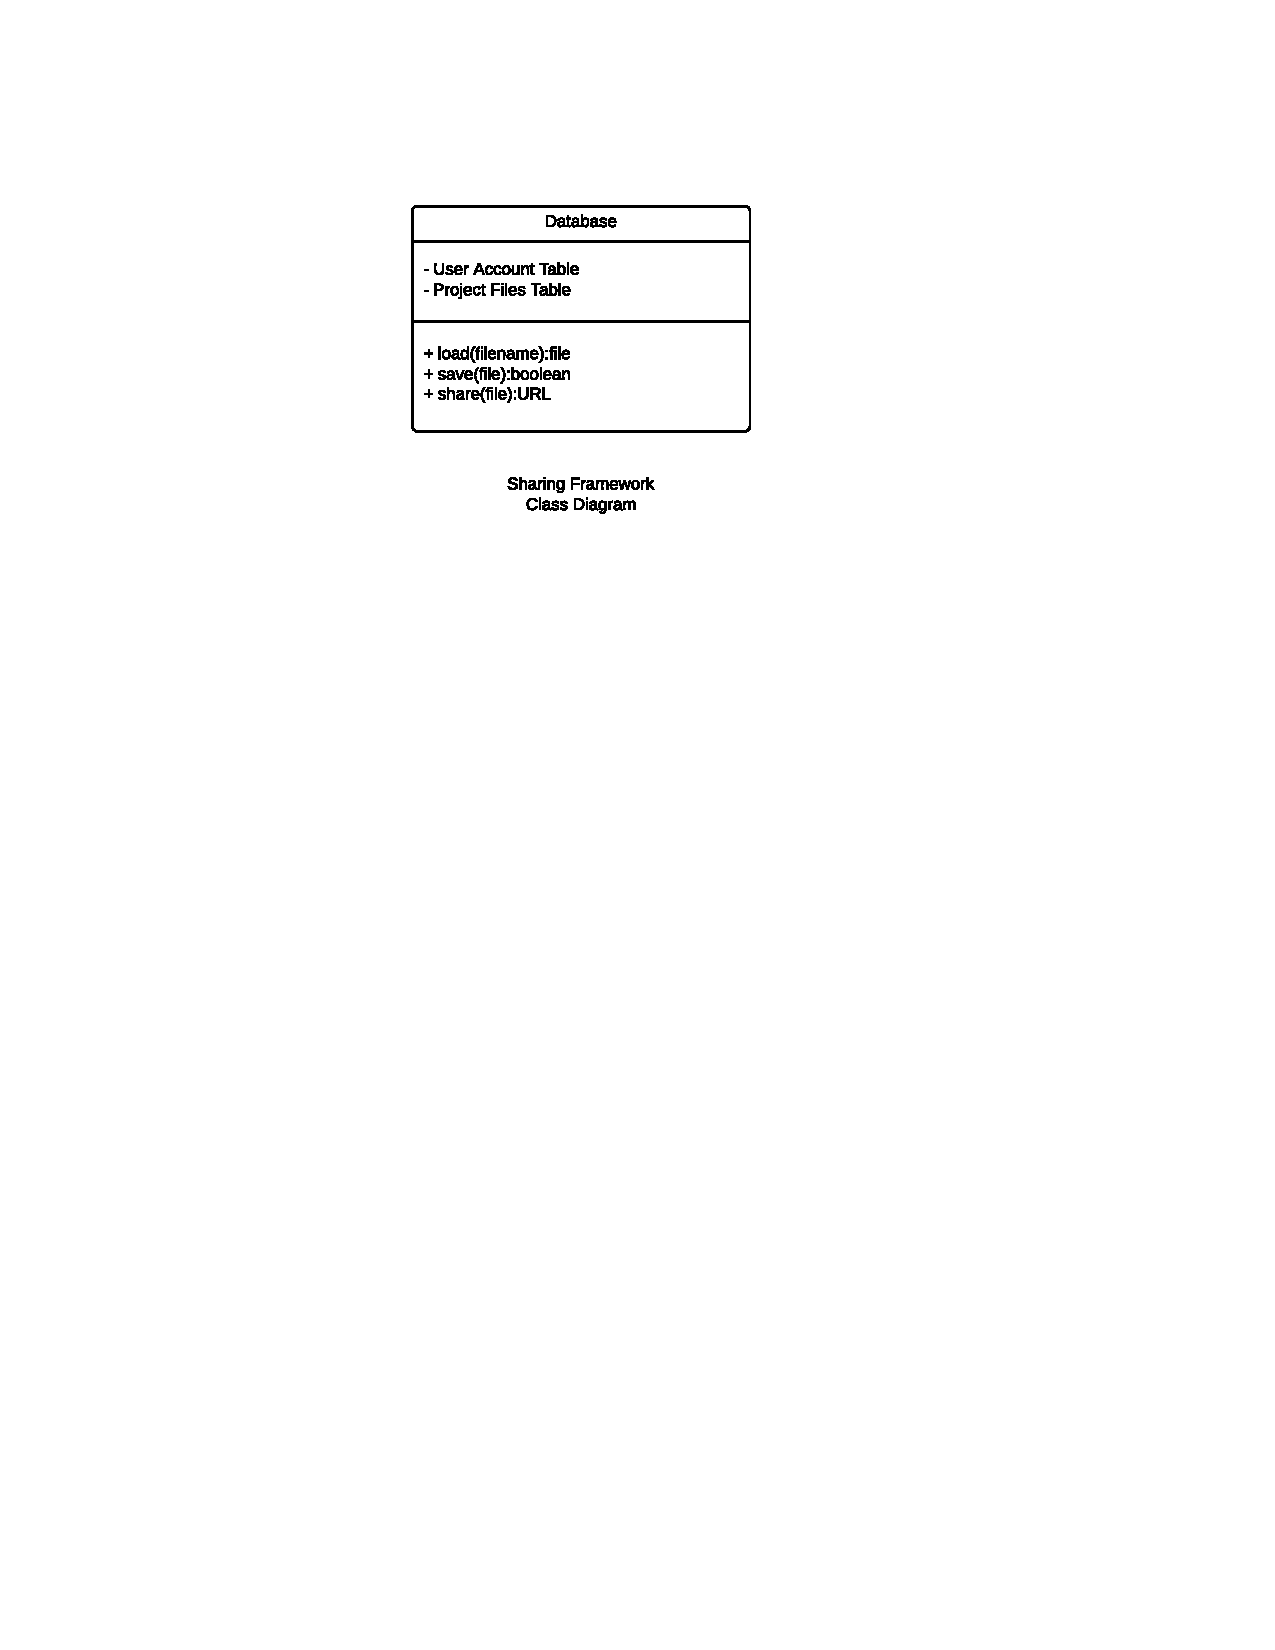
\includegraphics{sharingframework-uml.pdf}}
\end{figure}

\begin{figure}
 \centerline{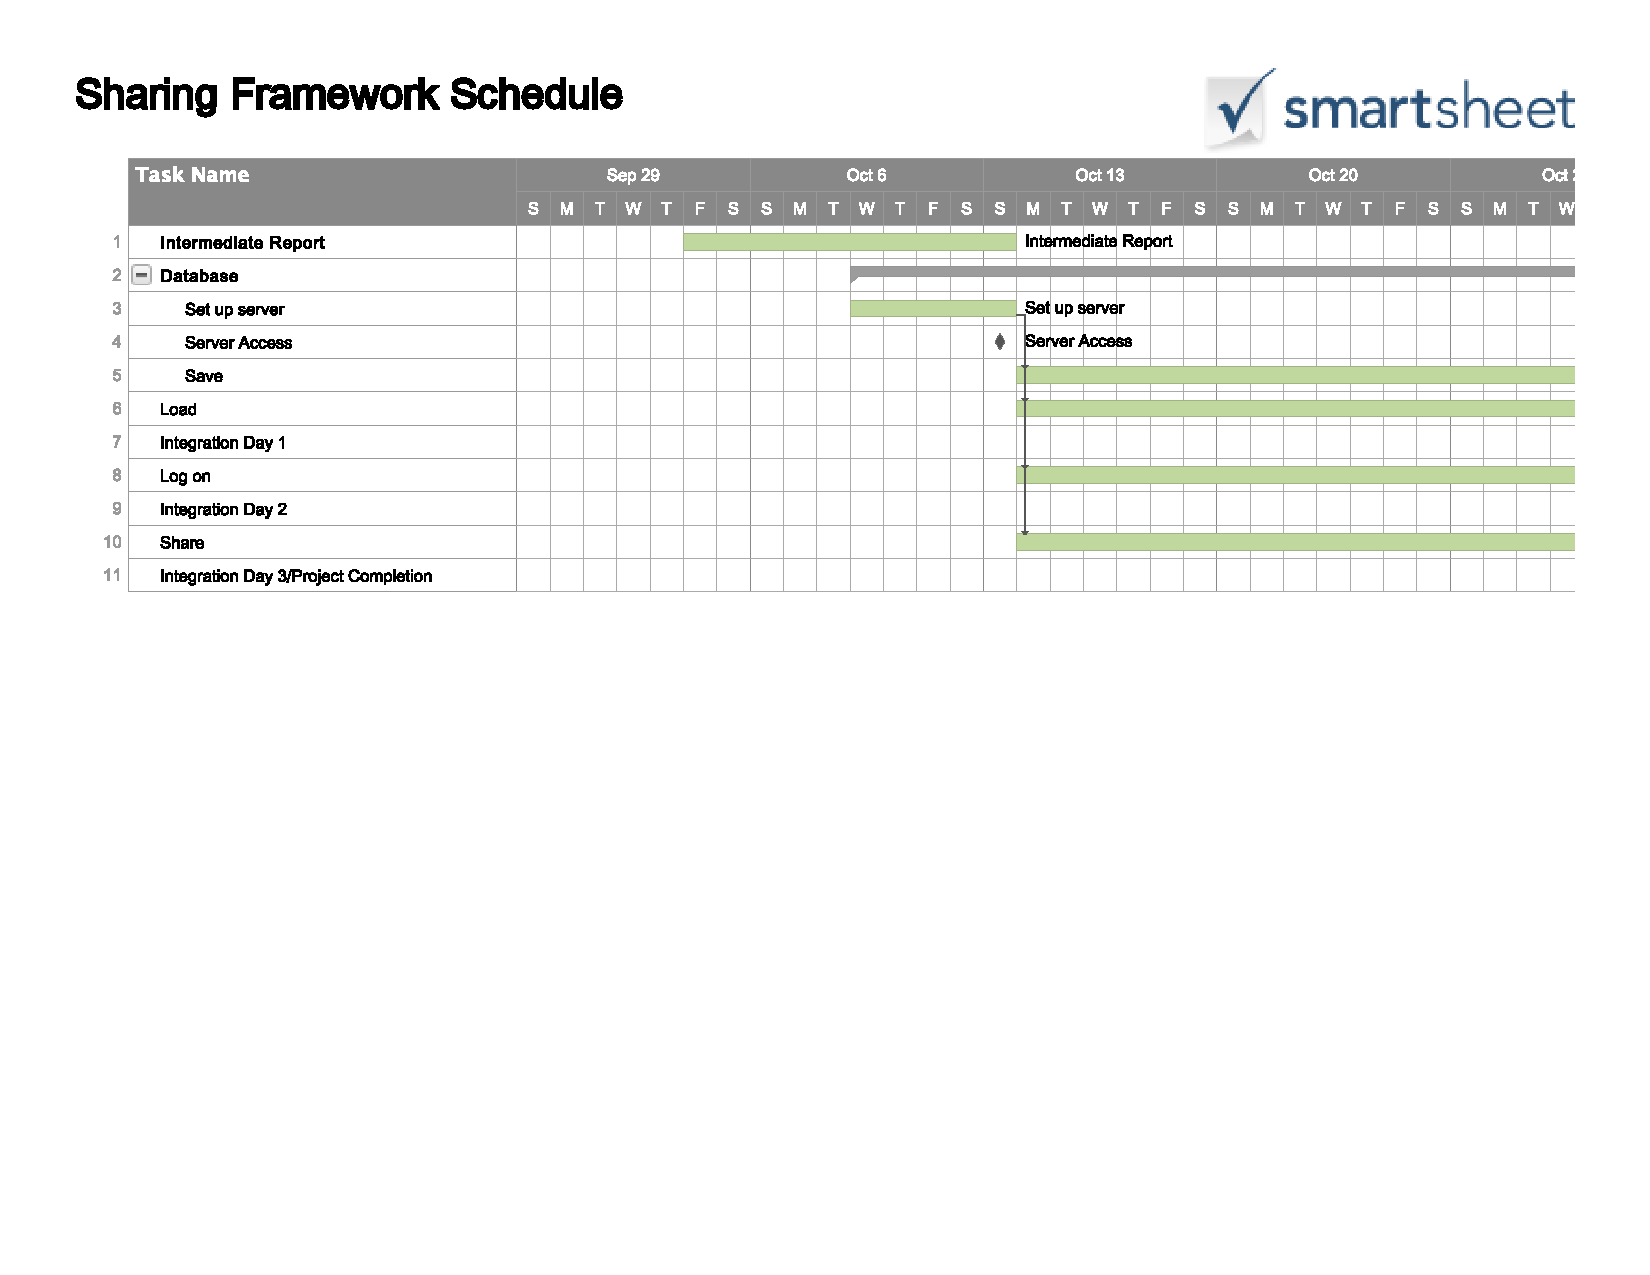
\includegraphics[scale=0.75]{sharingframework-sfs.pdf}}
\end{figure}

\begin{figure}
 \centerline{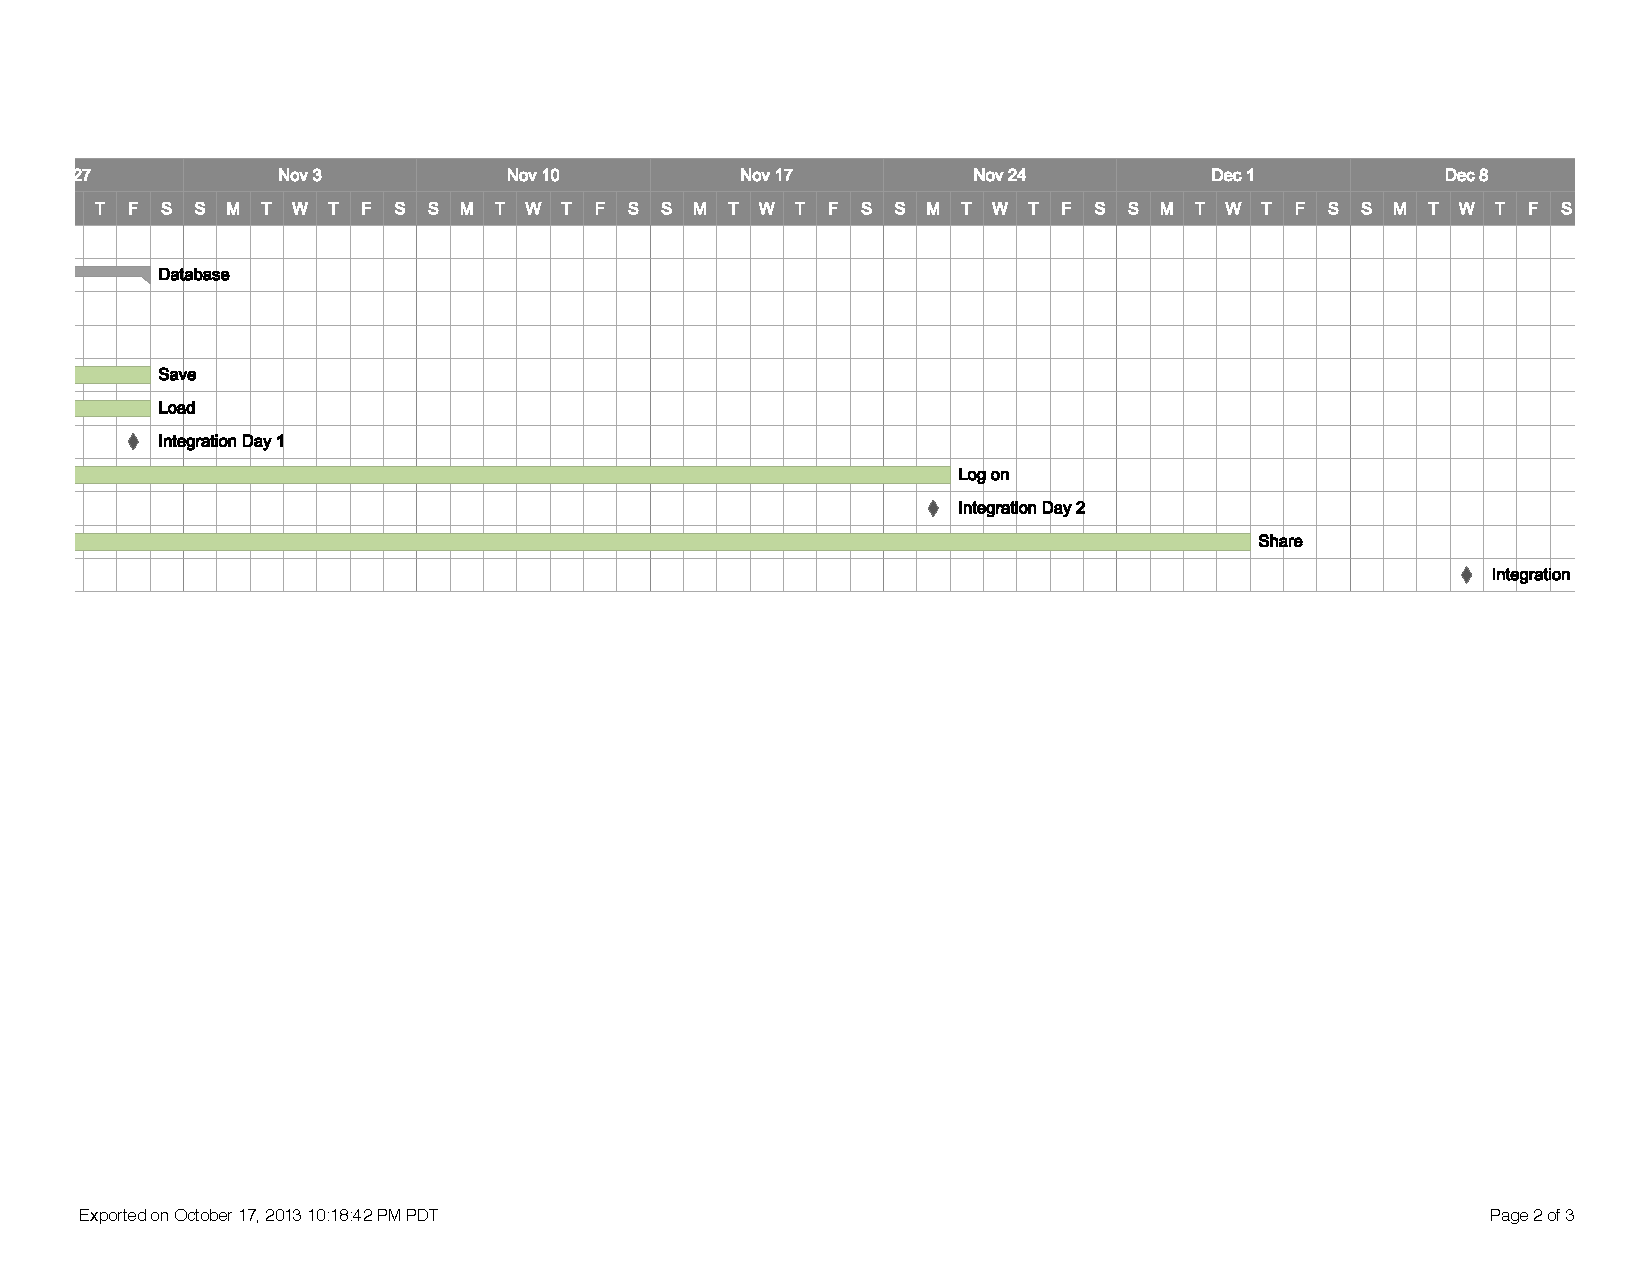
\includegraphics[scale=0.75]{sharingframework-sfs2.pdf}}
\end{figure}

\end{document}